\documentclass{article}
\usepackage[margin=0.5in]{geometry}
\usepackage[pdftex]{graphicx}
\usepackage{fullpage,graphicx,psfrag,url,caption}
\usepackage{amsmath,amsfonts,amssymb}
\usepackage{tikz}
\usepackage[europeanresistors,americaninductors]{circuitikz}
\usepackage{hyperref}
\setlength\parindent{0pt}

\newcommand{\sint}{sin(\theta/2)}
\newcommand{\cost}{cos(\theta/2)}
\newcommand{\lb}{\left[}
\newcommand{\rb}{\right]}
\newcommand{\parallelsum}{\mathbin{\|}}
\begin{document}

% this is a comment

\title{Revised Bluetooth commands for electrolyte and metabolite boards}

\author{Eric Wu}

\maketitle

\begin{itemize}

\item By default, the board is in sensing mode, and dumps out sensor readings and current values continuously in the format

    \begin{center}
        Sensor Ch1,Sensor Ch2,Current delivered,Current register
    \end{center}

    corresponding to the C formatting string ``\texttt{\%f,\%f,\%f,\%d\textbackslash n}". In sensing mode all of the sensor readings are valid, the current delivered should be very small, and the current register should be 0. The iontophoresis switches are open in sensing mode for safety.

\item Increasing the current register beyond 0 automatically puts the board into current monitoring mode. In this mode, the board dumps out sensor readings in the following format
    \begin{center}
        x,x,Current delivered,Current register
    \end{center}

    corresponding to the C formatting string ``\texttt{x,x,\%f,\%d\textbackslash n}". In current monitoring mode, the x's signify an invalid reading.

\item Lowering the current register to 0 or below 0 automatically puts the board back into sensing mode. Alternatively the command \texttt{0x40} will disable iontophoresis and puts the board back into sensing mode.

\item Each Bluetooth command is 8 bits, and is broken up in the following way:

    \bigskip

    \begin{centering}

    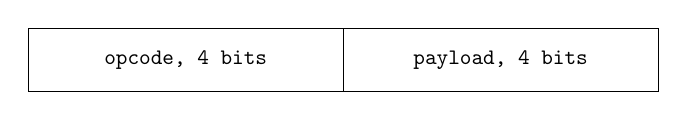
\begin{tikzpicture}[scale=0.8, transform shape]

        \draw (0,0) rectangle (5,1) node[midway] {\texttt{opcode, 4 bits}};
        \draw (5,0) rectangle (10, 1) node[midway] {\texttt{payload, 4 bits}};

    \end{tikzpicture}

    \end{centering}

\item The payload bits (ranging from \texttt{0x0} to \texttt{0xF}) are unsigned 4-bit integers

\item There is one 8-bit unsigned ``register" containing the iontophoresis PWM value, which corresponds to the 8-bit number used to set the iontophoresis current. \texttt{0} corresponds to no current, and \texttt{255} corresponds to maximum current. The current register-to-current transfer function is

    \begin{align*}
        I_{\textrm{out}} &= \frac{5 \textrm{r}}{255 \cdot 2085.31}
    \end{align*}

\item The 4-bit opcodes are

    \bigskip

    \begin{centering}

        \begin{tabular}{| l | l | p{6cm} |} \hline 
        Name & Hex & Function \\ \hline
        \texttt{DISABLE\_IONTOPHORESIS} & \texttt{0x4} & Disables iontophoresis, puts the board back into sensing mode. \\ \hline
        \texttt{ENABLE\_IONTOPHORESIS\_INCREMENT\_BY} & \texttt{0x5} & Adds the payload bits to the iontophoresis PWM value. Has overflow protection. Puts the board into iontophoresis mode automatically. \\ \hline
        \texttt{ENABLE\_IONTOPHORESIS\_DECREMENT\_BY} & \texttt{0x6} & Subtracts the payload from the iontophoresis PWM value. Has underflow protection. Takes the board into sensing mode automatically if PWM value reaches 0. \\ \hline
        \end{tabular}

    \end{centering}

\end{itemize}

\end{document}


